% =====================================================================
%  SchemaLens-Cassandra (TSDB / IoT-Benchmark) -- Versao ajustada v1
%  Compilar no Overleaf com pdfLaTeX. Tabelas em tables/ (geradas por
%  iot_v1/make_tables.py a partir dos dados brutos), figuras em figs/.
% =====================================================================
\documentclass[11pt,a4paper]{article}
\usepackage[T1]{fontenc}
\usepackage[utf8]{inputenc}
\usepackage{lmodern}
\IfFileExists{brazil.ldf}{\usepackage[brazil]{babel}}{}
\usepackage[a4paper,margin=2.2cm]{geometry}
\usepackage{amsmath,amssymb}
\usepackage{graphicx}
\usepackage{booktabs,tabularx,longtable,array}
\usepackage{float}
\usepackage[font=small,labelfont=bf]{caption}
\usepackage[table]{xcolor}
\usepackage{microtype}
\usepackage{fancyhdr}
\usepackage[colorlinks=true,linkcolor=blue!50!black,urlcolor=blue!50!black,citecolor=green!40!black]{hyperref}

\definecolor{boxbg}{RGB}{243,246,250}
\definecolor{warnbg}{RGB}{253,244,232}
\definecolor{okbg}{RGB}{236,247,240}
\newcommand{\caixa}[2][boxbg]{\par\smallskip\noindent\colorbox{#1}{\parbox{\dimexpr\linewidth-2\fboxsep}{#2}}\par\smallskip}
\newcommand{\just}[1]{\caixa{\textbf{Justificativa.} #1}}
\newcommand{\limit}[1]{\caixa[warnbg]{\textbf{Limitação.} #1}}
\newcolumntype{Y}{>{\raggedright\arraybackslash}X}
\newcommand{\envversion}{4.1.12}
\newcommand{\envdriver}{3.30.1}
\newcommand{\envpython}{3.12.3}
\newcommand{\envcpuset}{0-3}
\newcommand{\envmem}{6}
\newcommand{\envkernel}{7.0.0-38-generic}
\newcommand{\envrawrows}{28.800}
\newcommand{\envwindows}{5}
\newcommand{\envdiscarded}{0}
\newcommand{\envwinsec}{41}
\newcommand{\envrestart}{18}
\newcommand{\envguardsamples}{15}
\newcommand{\envstarted}{2026-11-17 17:50}
\newcommand{\envfinished}{2026-11-17 17:57}
\newcommand{\envothers}{5}
\newcommand{\envloadavg}{0{,}67}
\newcommand{\envnoise}{2{,}2\%}
\newcommand{\envnoiseq}{17{,}2\%}
\newcommand{\envsseven}{72/72}

\makeatletter\newcommand{\tabin}[1]{\@@input #1 }\makeatother

\pagestyle{fancy}\fancyhf{}
\lhead{\small SchemaLens--Cassandra (TSDB/IoT) --- versão ajustada v1}\rhead{\small Relatório de execução}
\cfoot{\thepage}

\title{\textbf{SchemaLens--Cassandra com o IoT-Benchmark}\\[4pt]
\large Versão ajustada: nova execução da fase de medição sob o protocolo comum v1\\
(correções da análise de consistência metodológica entre benchmarks)}
\author{Projeto SchemaLens / Cassandra}
\date{Execução: \envstarted--\envfinished{} UTC \quad--\quad relatório gerado em 17/11/2026}

\begin{document}
\maketitle

\begin{abstract}
\noindent A análise de consistência metodológica entre os quatro benchmarks do SchemaLens no Cassandra concluiu que a \emph{fase de projeto} é comum, mas a \emph{fase de execução} não: mudavam a versão do Cassandra, a métrica e a estatística, o número de deployments medidos, o controle de estado físico, a avaliação de preservação e as ablações. Este relatório documenta a versão ajustada do experimento IoT-Benchmark. Mantivemos congelada a fase de projeto da campanha B Rev3 (Stages 1--8, HBench de 3 deployments) e refizemos só a medição, sob um protocolo comum (v1) que valerá também para o TPCx-IoT e o TSBS. O protocolo fixa a imagem por digest (Cassandra \envversion), usa um container dedicado, mede os 6 deployments admissíveis e as 2 variantes de referência, faz 5 repetições com reinício a frio, decide pela média do mix uniforme com IC por bootstrap e piso de ruído por pares A/A, aplica gate de flush e guarda de isolamento, avalia Top-$k$, regret e retenção de Pareto, roda ablações das regras TS0--TS8/M1--M5 e de critérios do seletor e recalcula 10 gates de aceitação a partir dos dados brutos. Foram \envrawrows{} latências, todas conferidas pelo oráculo. \textbf{Resultado:} TS2-U, o rank 1 do seletor, é o melhor medido entre os 6 deployments admissíveis (média do mix de 4,15\,ms). Empata com a referência Q8-otimizada, que tem o mesmo DDL, e é 32\% mais rápido que TS0 e 67\% mais rápido que TS2-D, com piso de ruído de 2,2\%. Os resultados são Top-1, regret 0, retenção de Pareto de 100\% e $\tau=0{,}87$. As ablações mostram que só TS2 e M1 são decisivos: removê-los dá regret de 32\%. Os 10 gates e os 11 testes negativos passaram, e as 5 hipóteses pré-registradas foram confirmadas.

\end{abstract}

\tableofcontents
\newpage

% =====================================================================
\section{Resumo executivo}
% =====================================================================
\begin{enumerate}
\item \textbf{O que foi refeito.} Só a fase de medição, sob o protocolo comum v1: imagem Cassandra 4.1.12 fixada por digest, container dedicado com CPUs isoladas, 6 deployments admissíveis + 2 variantes de referência, 5 repetições com reinício a frio, \envrawrows{} latências conferidas pelo oráculo, gate de flush e guarda de isolamento (0 compactações, 0 janelas descartadas). A fase de projeto (HBench Rev3 da campanha B) ficou congelada e foi verificada byte a byte.
\item \textbf{Vencedor.} TS2-U (tabela larga sem bucket), o rank 1 do seletor, tem a menor média do mix: 4,145\,ms, IC [4,089; 4,199]. Empata com REF-Q8opt (razão 1,007; IC [0,990; 1,025]), o que é esperado, porque são o mesmo DDL com os mesmos planos. Fica à frente de TS0 (1,32$\times$) e de TS2-D (1,67$\times$), muito acima do piso de ruído (2,2\%). A referência original, com Q8 por varredura completa, é 1,20$\times$ mais lenta, e a diferença está toda no Q8 (24,9$\times$).
\item \textbf{Preservação (crítico 4 da análise).} Medindo o espaço inteiro, o HBench congelado acerta o Top-1 (estrito), tem regret 0 e retém 100\% da fronteira de Pareto medida (leitura, bytes, escrita), que é só TS2-U, e o $\tau$ de Kendall entre escore e medida é 0,87. Uma escolha aleatória de 3 em 6 teria regret esperado de 6,4\% e só 50\% de chance de conter o melhor.
\item \textbf{Ablações (importante 10).} Das 14 regras, 8 não ativam nesta carga (no-op). Só a remoção de \textbf{TS2} ou de \textbf{M1} piora o HBench (regret 31,6\%: perde-se TS2-U); a regra antiga ``TS0 obrigatória'' tem o mesmo efeito. TS0, TS1, TS4, TS5 e M3 não mudam a decisão. A salvaguarda de diversidade não é necessária para achar o melhor aqui, mas é ela que mantém TS0 e TS2-D como controles.
\item \textbf{Estatística comum (crítico 3).} Recalculada com a mesma estatística, a campanha B original dá a mesma ordenação (U $\approx$ REF-Q8opt $<$ REF $\approx$ TS0 $<$ TS2-D). A v1 reduz a largura do IC de $\approx$5,5\% para $\approx$2,7\% e separa REF de TS0, que na B se sobrepunham.
\item \textbf{O que não muda.} Neste workload estreito o vencedor continua sendo o desenho óbvio (TS2-U = tradução do modelo \texttt{table} do IoTDB). A v1 confirma, com rigor uniforme, a \emph{redução explicável sem perda do melhor}, mas não mostra ganho sobre a referência.
\end{enumerate}


% =====================================================================
\section{O que a análise de consistência apontou e o que foi ajustado}
% =====================================================================
A análise (\texttt{docs/Analise\_Consistencia\_Metodologica\_Benchmarks.pdf}) classificou 15 divergências. A Tabela~\ref{tab:ajustes} mostra como cada uma que se aplica ao IoT-Benchmark foi tratada nesta versão.

\begin{longtable}{@{}p{3.6cm}p{4.6cm}p{6.8cm}@{}}
\caption{Divergências da análise de consistência e tratamento na versão ajustada.}\label{tab:ajustes}\\
\toprule
\textbf{Divergência} & \textbf{Situação anterior (IoT)} & \textbf{Versão ajustada (protocolo v1)}\\\midrule\endfirsthead
\toprule\textbf{Divergência} & \textbf{Antes} & \textbf{v1}\\\midrule\endhead
Crítico 2 -- versão do Cassandra & tag flutuante \texttt{cassandra:4.1} (resolvia para 4.1.12), container compartilhado com outros experimentos & imagem fixada por digest \texttt{sha256:25f6a4d5\ldots} (release \envversion), container novo e dedicado, CPUs \envcpuset, \envmem{}\,GB, heap 2\,GB; cliente nas CPUs 8--11; preflight grava versão, digest, driver e ambiente\\
Crítico 3 -- métrica e estatística & p95 nearest rank de 60 amostras, uma sessão, sem IC & média, p50, p95 e p99; \textbf{métrica de decisão pré-declarada: média do mix uniforme}; IC 95\% por bootstrap estratificado; IC $t$ entre 5 repetições; contrastes pareados; piso de ruído por pares A/A\\
Crítico 4 -- avaliação de preservação & ``espaço pequeno demais para regret'' & \textbf{modo verification}: os 6 deployments admissíveis são medidos; Top-1, Top-3, near-best 5\%, regret, retenção de Pareto, $\tau$ de Kendall e comparação com escolha aleatória\\
Importante 8 -- tipo de carga & só leitura; escrita e armazenamento não medidos & tempo de carga e escritas físicas por deployment; bytes de SSTable por \texttt{nodetool tablestats}; Pareto medido em três objetivos\\
Importante 10 -- ablações & nenhuma & 14 ablações de regra (TS0--TS8, M1--M5) com o motor de ativação e o Stage 8 originais, mais 6 ablações de critério\\
Importante 11 -- estado físico, cache e isolamento & gate de flush só em S3; cache parcialmente frio em E6 & gate de flush antes de \emph{cada} repetição; reinício a frio do container; guarda de isolamento a cada 15\,s mais \texttt{compaction\_history}\\
Repetições e ordem & 60 rodadas AB/BA por consulta & 5 repetições $\times$ (10 aquecimentos + 60 rodadas); janela contínua; consultas e variantes em ordem sorteada, invertida nas rodadas pares\\
Aceitação & testes + auditoria Stage 7$\times$9 & 10 gates recalculados dos dados brutos + 10 testes negativos\\
Importantes 5, 6, 9 (custo, seletor, baseline) & próprios do benchmark & \textbf{não alterados} (fazem parte da fase de projeto congelada); o efeito deles agora é medido por Top-$k$, regret e ablações\\
\bottomrule
\end{longtable}

\just{A análise recomendou ``congelar um protocolo de execução v1 e reexecutar a fase de medição'', mantendo a fase de projeto, que já é consistente entre os TSDB (mesmo motor e mesmas regras, verificados por SHA-256). Refazer a fase de projeto mudaria a pergunta; manter o HBench congelado preserva o firewall entre seleção e medição.}

% =====================================================================
\section{Fase de projeto congelada (entrada da medição)}
% =====================================================================
\paragraph{Origem.} Campanha B Rev3 (05/11/2026): dados e objetos de consulta gerados pelo código Java oficial do IoT-Benchmark (commit \texttt{62e0dc10}), \texttt{DATA\_SEED}=531101, \texttt{QUERY\_SEED}=531107, 9 dispositivos, 2 sensores DOUBLE, 54.000 células (27.000 linhas largas, $\approx$20,8 dias), uma amostra de parâmetros por classe Q1--Q12, janela de consulta de 7 dias. A pasta \texttt{frozen\_design\_B/} é uma cópia byte a byte da campanha (verificada contra o original em 31 artefatos), e o código Rev3 confere com os hashes auditados.

\paragraph{Ativação e espaço admissível.} Cinco famílias ativam (TS0, TS1, TS2, TS4, TS5) e dois modificadores (M1, M3). O Stage 8 Rev3 enumera 6 coberturas completas (\{TS0, TS2-U, TS2-D\} $\times$ \{com, sem TS4\}); a fronteira de Pareto analítica tem só TS2-U, e a salvaguarda de diversidade estrutural acrescenta TS0 e TS2-D. HBench congelado (ordem do seletor): \textbf{TS2-U} (escore 1,000), \textbf{TS0} (2,024), \textbf{TS2-D} (2,039).

\paragraph{Pares A/A (trabalho idêntico).} Detectados automaticamente antes de medir: TS2-U $\equiv$ TS2-U+TS4 e TS2-D $\equiv$ TS2-D+TS4 (as rotas não usam TS4, porque Q8 é atendida por leitura descendente na tabela larga), e TS2-U $\equiv$ REF-Q8opt (mesmo DDL e mesmos planos em keyspaces diferentes). Esses pares definem o piso de ruído.

\paragraph{Pré-registro.} \texttt{PREREGISTRATION\_IOT\_V1.json} grava os SHA-256 do código de medição, do protocolo e dos 31 artefatos de projeto, as 8 variantes, os pares A/A, as sementes e as hipóteses H1--H5. Foi gravado em modo exclusivo antes da medição. Um primeiro pré-registro foi substituído antes de qualquer medição oficial, porque a normalização de DDL não reconheceu o par TS2-U $\equiv$ REF-Q8opt; a versão superada e a nota estão em \texttt{preregistration\_history/}.

% =====================================================================
\section{Protocolo v1 aplicado}
% =====================================================================
\begin{table}[H]\centering\small
\caption{Execução realizada.}
\begin{tabularx}{\linewidth}{@{}lY@{}}\toprule
Cassandra & \envversion, nó único, RF=1, imagem por digest, container \texttt{sl\_v1\_iot\_cassandra} (porta 9061), CPUs \envcpuset, \envmem\,GB\\
Cliente & Python \envpython, \texttt{cassandra-driver} \envdriver, afinidade CPUs 8--11; kernel \envkernel\\
Host & \envothers{} outros containers ativos (ociosos), loadavg no preflight \envloadavg\\
Variantes & 6 coberturas admissíveis (keyspace próprio cada) + REF e REF-Q8opt (mesma tabela de referência, planos diferentes)\\
Carga & carregador sequencial original (\texttt{\_materialize}/\texttt{load\_wide}), cronometrado por deployment; \texttt{nodetool flush}; espera de compactações\\
Repetições & 5 $\times$ [reinício a frio (média \envrestart\,s) $\rightarrow$ gate de flush $\rightarrow$ pré-checagem do oráculo em 96 rotas $\rightarrow$ 10 aquecimentos $\rightarrow$ 60 rodadas]; janela média \envwinsec\,s\\
Isolamento & \envguardsamples{} amostras de \texttt{system\_views.sstable\_tasks}; \texttt{compaction\_history} antes/depois; janelas descartadas: \envdiscarded\\
Volume & \envrawrows{} latências cronometradas ($5\times60\times12\times8$), todas conferidas pelo oráculo\\
\bottomrule\end{tabularx}\end{table}

\just{O reinício a frio entre repetições descarta caches da JVM (key cache, chunk cache, estado do JIT) e torna as repetições estatisticamente independentes; o gate garante que todas as variantes leem de SSTable, e não de memtable. Isso corrige a assimetria física observada em S2. A média do mix foi escolhida como métrica de decisão antes de medir porque o p95 de poucas dezenas de amostras se mostrou instável em consultas de 1--5\,ms (Fase 4) e porque a média é aditiva num mix, que é o critério do RUBiS V9.}
\limit{Os dados (\,$\approx$3\,MB) cabem inteiros no page cache do host, então ``frio'' aqui significa JVM e caches do Cassandra frios, não disco frio. A latência é ponta a ponta no cliente Python (driver + pós-processamento).}

% =====================================================================
\section{Resultados}
% =====================================================================
\subsection{Média do mix (métrica de decisão)}
\begin{table}[H]\centering\small
\caption{Métricas do mix uniforme Q1--Q12 (ms), ordenadas pela média. IC boot: bootstrap estratificado (2.000 reamostras); IC $t$: sobre as 5 médias por repetição; CV rep: variação entre repetições.}
\resizebox{\linewidth}{!}{\begin{tabular}{@{}llrcccrrr@{}}\toprule
Variante & Papel & Média & IC 95\% boot & IC 95\% $t$ & p95 médio & p50 & p99 & CV rep \%\\\midrule
\tabin{tables/t_mix.tex}
\bottomrule\end{tabular}}\end{table}

\begin{figure}[H]\centering
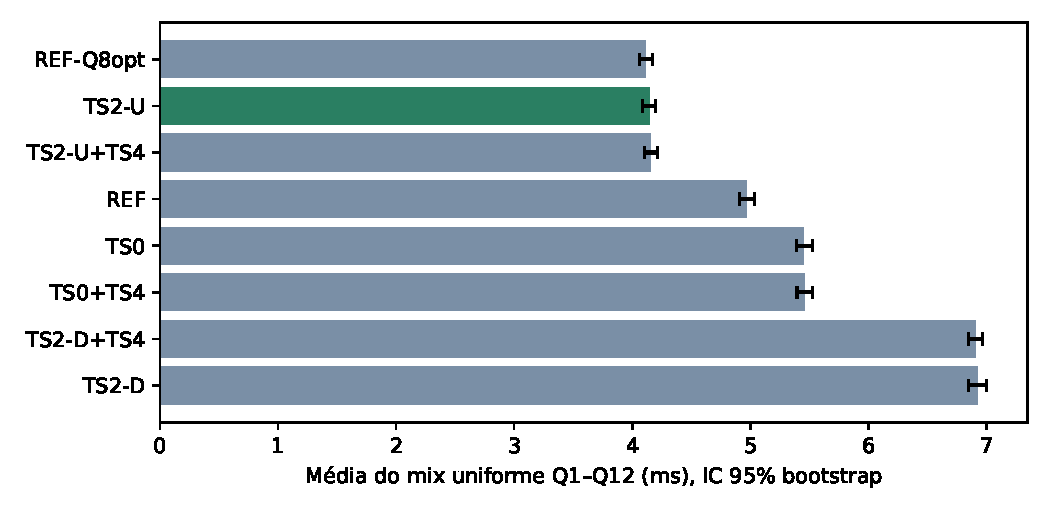
\includegraphics[width=0.8\linewidth]{figs/fig_v1_mix.pdf}
\caption{Média do mix com IC 95\% (bootstrap). Verde: rank 1 do seletor (TS2-U).}
\end{figure}

\subsection{Piso de ruído e contrastes pareados}
\begin{table}[H]\centering\small
\caption{Pares A/A (trabalho idêntico em keyspaces diferentes). Piso de ruído = maior quantil 95\% de $|\ln \text{razão}|$ = \envnoise{}.}
\begin{tabular}{@{}lccc@{}}\toprule
Par & Razão das médias & IC 95\% & q95 $|\ln r|$\\\midrule
\tabin{tables/t_noise.tex}
\bottomrule\end{tabular}\end{table}

\begin{longtable}{@{}llccl@{}}
\caption{Contrastes pareados da média do mix (razão A/B). Empate: o IC contém 1 ou $|\ln r|$ fica abaixo do piso de ruído.}\\
\toprule A & B & Razão A/B & IC 95\% & Veredito\\\midrule\endhead
\tabin{tables/t_contrasts.tex}
\bottomrule
\end{longtable}

\subsection{Por classe de consulta}
\begin{longtable}{@{}lrrrrrr@{}}
\caption{Média e p95 de TS2-U (ms) e razão das médias de outras variantes sobre TS2-U, por classe. Em negrito: IC que exclui 1 e $|\ln r|$ acima do piso de ruído por classe (\envnoiseq{}, derivado do par A/A REF-Q8opt $\equiv$ TS2-U).}\\
\toprule Q & média U & p95 U & TS2-D/U & TS0/U & REF/U & REF-Q8opt/U\\\midrule\endhead
\tabin{tables/t_perquery.tex}
\bottomrule
\end{longtable}
\begin{figure}[H]\centering
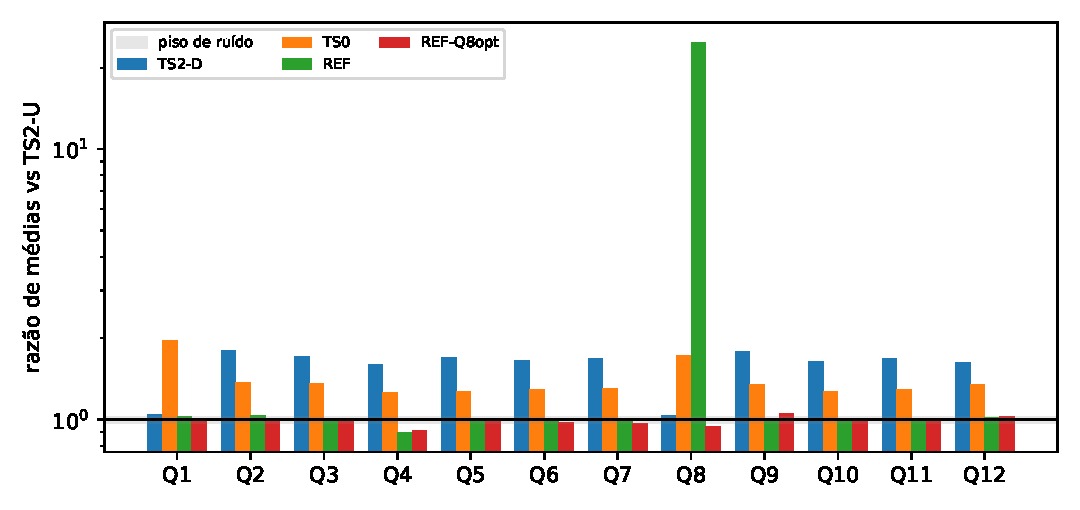
\includegraphics[width=0.9\linewidth]{figs/fig_v1_perquery.pdf}
\caption{Razão das médias por classe em relação a TS2-U (escala log). Faixa cinza: piso de ruído.}
\end{figure}
\paragraph{Leitura.} A penalidade de TS2-D aparece em todas as classes que leem intervalos (1,60--1,80$\times$), porque o bucket diário multiplica as chamadas CQL (uma por dia da janela de 7 dias). Q1 (ponto) e Q8 (último valor) não mudam. TS0 paga uma partição por sensor: Q1 sai 1,96$\times$ mais lento e Q8 1,72$\times$. A referência original só perde no Q8 (24,9$\times$, varredura completa); com o Q8 otimizado ela é indistinguível de TS2-U em todas as classes. \textbf{Observação metodológica:} no par A/A REF-Q8opt $\equiv$ TS2-U as razões por classe variam de 0,91 a 1,05 (por exemplo, Q4), embora o trabalho seja idêntico. Por isso diferenças de até $\approx$17\% numa classe isolada não são interpretáveis, e a decisão é tomada no mix, cujo piso é de 2,2\%.


\subsection{Armazenamento e escrita (objetivos do Pareto)}
\begin{table}[H]\centering\small
\caption{Custos físicos medidos por deployment. Armazenamento: \texttt{Space used (live)} após flush; escrita: carregador sequencial (mesmo para todos). Proxy: estimativa do Stage 7.}
\resizebox{\linewidth}{!}{\begin{tabular}{@{}llrrrr@{}}\toprule
Variante & Tabelas & KiB em disco & Carga (s) & Escritas & Proxy (KiB)\\\midrule
\tabin{tables/t_cost.tex}
\bottomrule\end{tabular}}\end{table}
\paragraph{Leitura.} TS0 ocupa 1,8$\times$ mais disco (uma linha por célula) e leva 2,2$\times$ mais tempo de carga (54 mil escritas contra 27 mil). TS4 custa só $\approx$6\,KiB e 18 escritas. TS2-D ocupa 2,3\% mais que TS2-U (189 partições contra 9). A fronteira de Pareto medida nos três objetivos tem um único ponto, TS2-U, que domina os demais em leitura, bytes e escrita. A única exceção é REF, que tem o mesmo DDL e fica fora do espaço admissível. Os proxies de armazenamento do Stage 7 superestimam os bytes reais em $\approx$6$\times$ (o Cassandra comprime), mas preservam a ordem TS0 $>$ TS2.


\subsection{Previsão estrutural (Stage 7 $\times$ Stage 9)}
Chamadas \texttt{execute} e linhas iteradas previstas pelo Stage 7 coincidiram com as observadas em \textbf{\envsseven{}} rotas (6 deployments $\times$ 12 consultas), em todas as repetições.

\subsection{Avaliação do método no espaço admissível}
\begin{table}[H]\centering\small
\caption{Indicadores de preservação (modo verification, 6 deployments medidos).}
\begin{tabularx}{\linewidth}{@{}lY@{}}\toprule
\tabin{tables/t_method.tex}
\bottomrule\end{tabularx}\end{table}
\paragraph{Leitura.} Com o espaço inteiro medido, o HBench congelado preserva o melhor (Top-1 estrito) com redução de 50\%. A ordenação do seletor (U $<$ TS0 $<$ D) coincide com a medida. O $\tau=0{,}87$ não chega a 1 só porque o seletor põe as variantes com TS4 marginalmente atrás das sem TS4 (escores 1,0001 contra 1,0000), e na medida elas empatam. O espaço é pequeno (6), então o resultado vale como verificação de consistência, não como demonstração de poder de redução em espaço rico.


\subsection{Ablações}
\begin{longtable}{@{}p{4.3cm}p{4.2cm}rcp{3.6cm}@{}}
\caption{Ablações de regra (motor de ativação original, sem a regra) e de critério do seletor. Regret e near-best calculados com as medições do modo verification.}\\
\toprule Ablação & HBench resultante & Regret & Near-best 5\% & Observação\\\midrule\endhead
\tabin{tables/t_ablation.tex}
\bottomrule
\end{longtable}
\paragraph{Leitura.} As ablações mostram que a decisão depende de duas regras: a ativação de TS2 (colocalização multimétrica) e a do modificador M1 (granularidade do bucket, que materializa TS2-U). Sem qualquer uma delas, o HBench perde o melhor deployment e o regret medido sobe a 31,6\%, pior que a escolha aleatória (6,4\% esperado). As regras de TS3, TS6, TS7, TS8, M2, M4 e M5 não ativam nesta carga, então não se pode afirmar nada sobre a contribuição delas aqui; isso reforça a limitação de diversidade do workload. Sem Pareto, sem diversidade ou com $k=1$ o melhor também é encontrado, porque o escore ponderado já põe TS2-U em primeiro.


\subsection{Campanha B original recalculada com a estatística v1}
A estatística comum também foi aplicada às latências brutas já gravadas da campanha B confirmatória (60 rodadas, uma sessão, sem reinício), sem medir de novo, como recomendou a análise (prioridade 3).
\begin{table}[H]\centering\small
\caption{Campanha B (05/11) recalculada $\times$ v1 (17/11). Mesmo HBench, mesmos dados, mesmas consultas.}
\begin{tabular}{@{}lrrcrr@{}}\toprule
 & \multicolumn{3}{c}{B original (recalculada)} & \multicolumn{2}{c}{v1}\\\cmidrule(lr){2-4}\cmidrule(lr){5-6}
Variante & p95 médio & Média & IC 95\% & Média & p95 médio\\\midrule
\tabin{tables/t_legacy.tex}
\bottomrule\end{tabular}\end{table}
\paragraph{Leitura.} A ordenação é a mesma nas duas execuções. As médias absolutas da v1 são $\approx$20\% menores, efeito de CPUs isoladas, container dedicado e aquecimento por repetição. Os IC da v1 são cerca de metade da largura. Pela métrica antiga (p95 médio), TS2-U e REF-Q8opt também empatam nas duas. A conclusão da campanha B se mantém, agora com estatística comparável à dos demais benchmarks.


% =====================================================================
\section{Hipóteses pré-registradas}
% =====================================================================
\begin{longtable}{@{}p{0.7cm}p{6.2cm}p{1.9cm}p{5.8cm}@{}}
\toprule & Hipótese & Resultado & Evidência\\\midrule\endhead
\tabin{tables/t_hyp.tex}
\bottomrule
\end{longtable}

% =====================================================================
\section{Aceitação}
% =====================================================================
\begin{minipage}[t]{0.48\linewidth}\centering\small
\begin{tabular}[t]{@{}lc@{}}\toprule Gate (dados brutos) & \\\midrule
\tabin{tables/t_gates.tex}
\bottomrule\end{tabular}
\end{minipage}\hfill
\begin{minipage}[t]{0.5\linewidth}\centering\small
\begin{tabular}[t]{@{}lc@{}}\toprule Teste negativo & \\\midrule
\tabin{tables/t_neg.tex}
\bottomrule\end{tabular}
\end{minipage}

\medskip
Todos os gates foram recalculados a partir de \texttt{raw\_latencies.csv} e \texttt{manifest.json}. A razão máxima/mínima de posições na ordem contrabalançada foi 1,18. Os testes negativos comprovam que o pipeline recusa ou detecta: dado adulterado, código alterado depois do pré-registro, resposta errada ou incompleta, keyspace inseguro, amostra faltante, compactação durante a janela, memtable não vazia ou ausência de SSTable, sobrescrita do pré-registro e reuso de container. \textbf{Status: ACEITO.}


% =====================================================================
\section{O que muda nas conclusões do IoT-Benchmark}
% =====================================================================
\begin{enumerate}
\item \textbf{Comparabilidade.} O IoT-Benchmark passa a ter fase de medição idêntica, em protocolo, à que será aplicada ao TPCx-IoT e ao TSBS: mesma imagem, mesmas métricas, mesma estatística, mesmo controle físico e mesmos indicadores de preservação. A afirmação ``esquema A melhor que B'' passa a ter o mesmo critério (média do mix, IC bootstrap, piso A/A).
\item \textbf{Conclusões anteriores confirmadas:} TS2-U é a melhor escolha para esta carga; o bucket diário custa uma chamada por dia; o seletor ordena corretamente; e o vencedor coincide com a referência (mesmo DDL).
\item \textbf{Conclusões novas:} (i) o HBench preserva o melhor e toda a fronteira de Pareto medida (antes ``espaço pequeno demais''); (ii) a decisão depende das regras TS2 e M1, e a ablação quantifica isso (regret de 31,6\% sem elas); (iii) TS0 e TS2-D também perdem em armazenamento e em escrita, então o Pareto de três objetivos tem um único ponto; (iv) diferenças por classe abaixo de $\approx$17\% estão dentro do ruído A/A.
\item \textbf{Para o artigo.} Escrever ``redução explicável que preservou o melhor deployment e a fronteira de Pareto medida (6 $\rightarrow$ 3, regret 0), sob o protocolo comum v1''. Não afirmar ganho de desempenho sobre a referência.
\end{enumerate}


% =====================================================================
\section{Limitações e ameaças à validade}
% =====================================================================
\begin{itemize}
\item \textbf{Interna.} Latência no cliente Python (driver + pós-processamento); nó único; os dados cabem no page cache do host (frio = JVM/caches do Cassandra); outros containers estavam ativos, embora ociosos e em outras CPUs. O Q1 devolve resposta vazia, porque o ponto amostrado pelo gerador Java não coincide com um timestamp armazenado, então a checagem de corretude do Q1 só confirma a ausência de linhas.
\item \textbf{Construto.} A média do mix uniforme pressupõe frequências iguais (\texttt{OPERATION\_PROPORTION} não é reproduzido); ``escrita'' é o carregador sequencial, não a ingestão concorrente; armazenamento é \texttt{Space used (live)} após flush, sem compactação de longo prazo.
\item \textbf{Externa.} Um workload estreito (2 sensores DOUBLE, 1 dispositivo por consulta, 54 mil células); o espaço admissível tem só 6 deployments, então Top-$k$ e regret são pouco discriminantes (escolher 3 de 6 ao acaso já contém o melhor com probabilidade 0,5).
\item \textbf{Conclusão.} O HBench e as regras foram desenvolvidos iterativamente com dados anteriores (V3 $\rightarrow$ Rev3). A v1 mede de novo uma seleção congelada; não é um holdout novo de dados.
\item \textbf{Não harmonizado.} Modelo de custo, seletor e natureza do baseline seguem próprios do benchmark (importantes 5, 6 e 9).
\end{itemize}

% =====================================================================
\appendix
\section{Reprodução passo a passo}
\begin{verbatim}
cd versao_ajustada/iot_benchmark_tsdb
python3 -m venv ../.venv && ../.venv/bin/pip install cassandra-driver numpy matplotlib
./run_all.sh smoke      # opcional, container descartavel
./run_all.sh freeze     # pre-registro (exclusivo)
./run_all.sh measure    # ~10 min -> outputs/v1_run1/
./run_all.sh analyze    # metricas, bootstrap, Top-k/regret, figuras
./run_all.sh ablation   # ablacoes (offline)
./run_all.sh accept     # gates + testes negativos
../.venv/bin/python iot_v1/make_tables.py --run outputs/v1_run1
./run_all.sh report     # compila este PDF
\end{verbatim}

\section{Artefatos}
\begin{longtable}{@{}p{6cm}p{8.6cm}@{}}\toprule
\texttt{../common/protocol\_v1.json} & protocolo comum congelado\\
\texttt{PREREGISTRATION\_IOT\_V1.json} & pré-registro (hashes, variantes, A/A, H1--H5)\\
\texttt{frozen\_design\_B/} & fase de projeto congelada (campanha B Rev3)\\
\texttt{outputs/v1\_run1/raw\_latencies.csv} & \envrawrows{} latências com chamadas, linhas, plano e oráculo\\
\texttt{outputs/v1\_run1/manifest.json} & preflight, por repetição: reinício, gate, guarda, janela\\
\texttt{outputs/v1\_run1/load.csv}, \texttt{storage\_tables.csv} & escrita e armazenamento\\
\texttt{outputs/v1\_run1/analysis/} & todas as tabelas deste relatório em CSV/JSON\\\bottomrule
\end{longtable}

\begin{thebibliography}{9}\small
\bibitem{iotbench} thulab/iot-benchmark. \url{https://github.com/thulab/iot-benchmark}, commit \texttt{62e0dc10}.
\bibitem{efron} B.~Efron, R.~J.~Tibshirani. \emph{An Introduction to the Bootstrap}. Chapman \& Hall, 1993.
\bibitem{hyndman} R.~J.~Hyndman, Y.~Fan. Sample quantiles in statistical packages. \emph{The American Statistician}, 50(4), 1996.
\bibitem{nosek} B.~A.~Nosek et al. The preregistration revolution. \emph{PNAS}, 115(11), 2018.
\bibitem{kalibera} T.~Kalibera, R.~Jones. Rigorous benchmarking in reasonable time. \emph{ISMM}, 2013.
\end{thebibliography}
\end{document}
